\documentclass[ignorenonframetext,]{beamer}
\setbeamertemplate{caption}[numbered]
\setbeamertemplate{caption label separator}{: }
\setbeamercolor{caption name}{fg=normal text.fg}
\beamertemplatenavigationsymbolsempty
\usepackage{lmodern}
\usepackage{amssymb,amsmath}
\usepackage{ifxetex,ifluatex}
\usepackage{fixltx2e} % provides \textsubscript
\ifnum 0\ifxetex 1\fi\ifluatex 1\fi=0 % if pdftex
\usepackage[T1]{fontenc}
\usepackage[utf8]{inputenc}
\else % if luatex or xelatex
\ifxetex
\usepackage{mathspec}
\else
\usepackage{fontspec}
\fi
\defaultfontfeatures{Ligatures=TeX,Scale=MatchLowercase}
\fi
% use upquote if available, for straight quotes in verbatim environments
\IfFileExists{upquote.sty}{\usepackage{upquote}}{}
% use microtype if available
\IfFileExists{microtype.sty}{%
\usepackage{microtype}
\UseMicrotypeSet[protrusion]{basicmath} % disable protrusion for tt fonts
}{}
\newif\ifbibliography

% Prevent slide breaks in the middle of a paragraph:
\widowpenalties 1 10000
\raggedbottom

\AtBeginPart{
\let\insertpartnumber\relax
\let\partname\relax
\frame{\partpage}
}
\AtBeginSection{
\ifbibliography
\else
\let\insertsectionnumber\relax
\let\sectionname\relax
\frame{\sectionpage}
\fi
}
\AtBeginSubsection{
\let\insertsubsectionnumber\relax
\let\subsectionname\relax
\frame{\subsectionpage}
}

\setlength{\parindent}{0pt}
\setlength{\parskip}{6pt plus 2pt minus 1pt}
\setlength{\emergencystretch}{3em}  % prevent overfull lines
\providecommand{\tightlist}{%
\setlength{\itemsep}{0pt}\setlength{\parskip}{0pt}}
\setcounter{secnumdepth}{0}

\title{Data-driven Temporal Phenotyping\\
of the GCAT Cohort from Electronic Health Records}
\author{Xavier Duran-Albareda\\
GCAT Genomes for Life\\
Institut de Recerca Germans Trias i Pujol (IGTP)}
\date{FI-2017 AGAUR\\
October 28\textsuperscript{th}, 2016}

\begin{document}
\frame{\titlepage}

\begin{frame}{A Cohort Study of the Genomes of Catalonia}


\includegraphics[keepaspectratio,width=0.2\textwidth]{images/logo-GCAT.png}

\begin{itemize}
\tightlist
\item
  Genomic population-based cohort
\item
  25.000 participants by 2018
\item
  General, asymptomatic population
\item
  Analyze genomics and health interplay in the next 20 years
\end{itemize}


\includegraphics[keepaspectratio,width=0.5\textwidth]{images/chronic_disease_epidemiology_group_image.jpg}

\end{frame}

\begin{frame}{Cohort studies linked to Electronic Health Records}

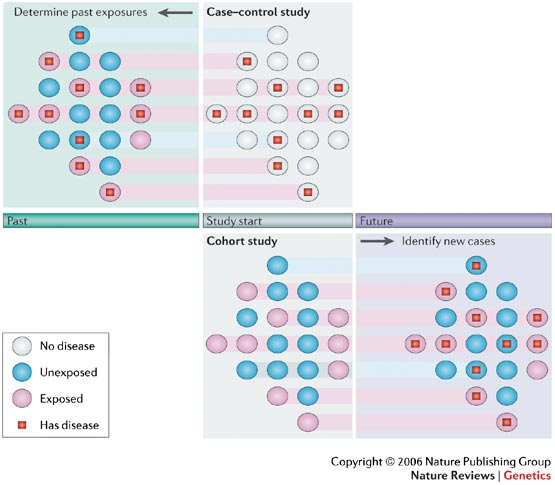
\includegraphics[keepaspectratio,width=0.5\textwidth]{images/case_control_nature.jpeg}

\begin{itemize}
\tightlist
\item
  Identify the \textbf{genomic basis} of \textbf{common disorders}
\item
  \textbf{Electronic Health Records} are the major source of phenotype
  data available
\item
  From hypothesis-driven to \textbf{data-driven} phenotyping
\end{itemize}

\end{frame}

\begin{frame}{Temporal disease trajectories and disease clusters}

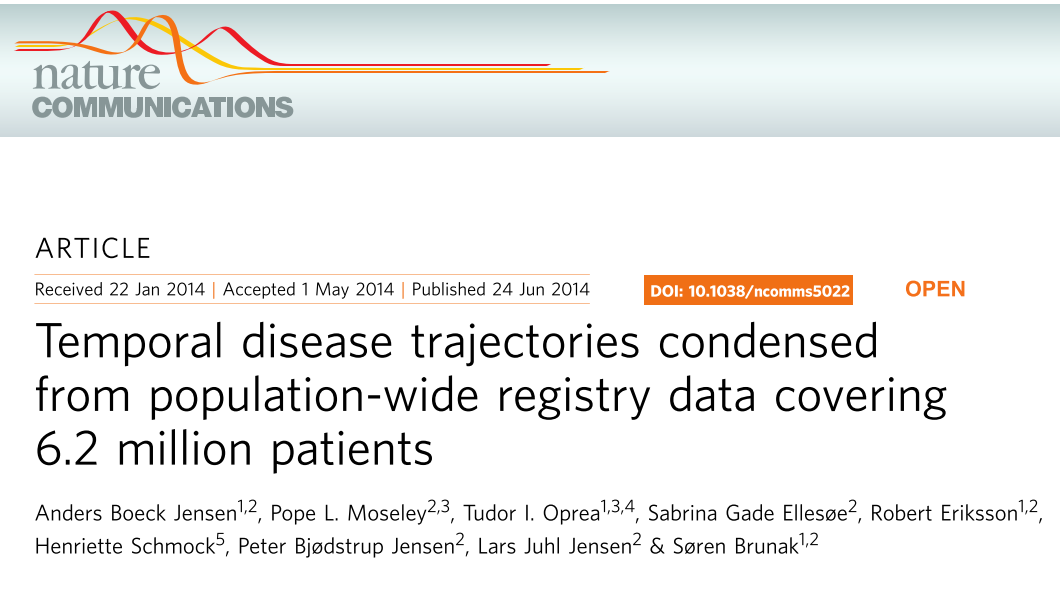
\includegraphics[keepaspectratio,width=0.5\textwidth]{images/trajectories.png}

\begin{figure}[t!]
  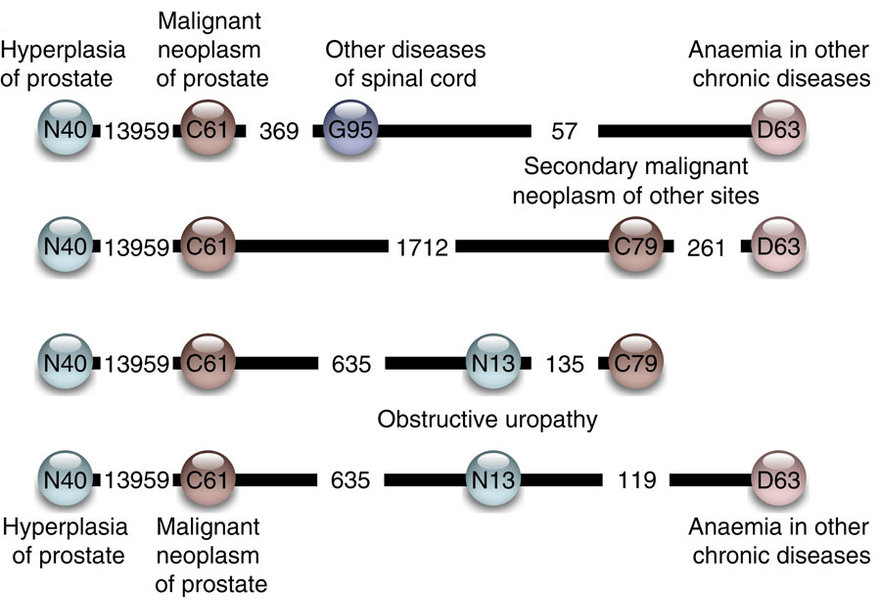
\includegraphics[keepaspectratio,width=0.5\textwidth]{images/ncomms5022-f11.png}
  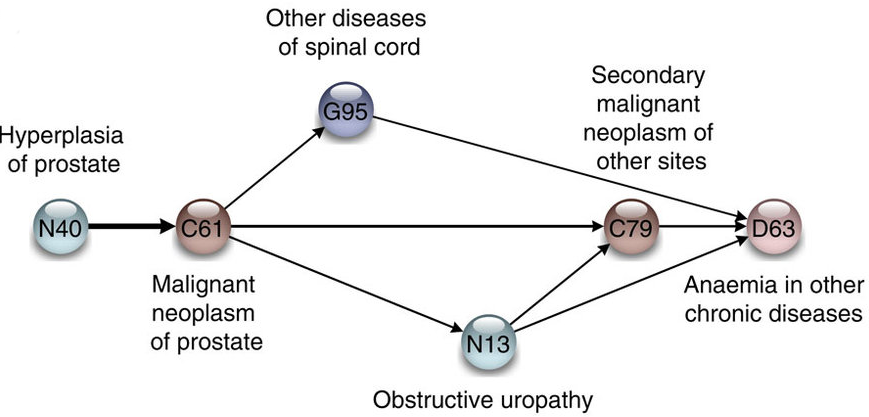
\includegraphics[keepaspectratio,width=0.5\textwidth]{images/ncomms5022-f12.png}
\end{figure}

\end{frame}

\begin{frame}{GCAT Snapshot and the Diseasome}

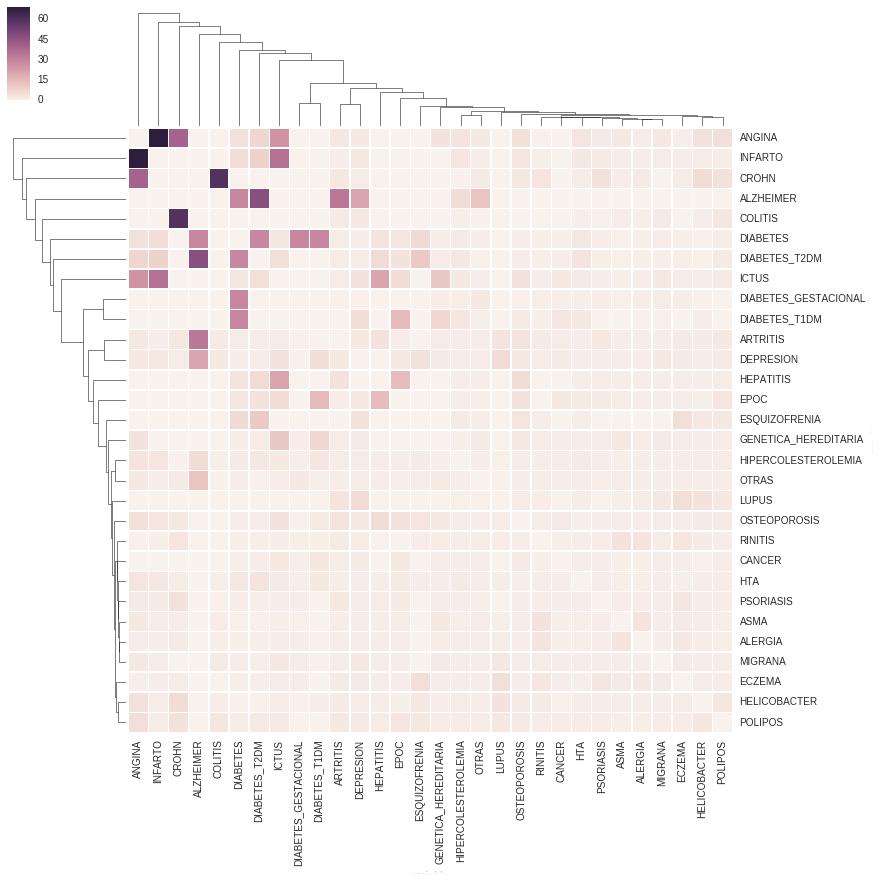
\includegraphics[keepaspectratio,width=0.5\textwidth]{images/relative_risk.png}
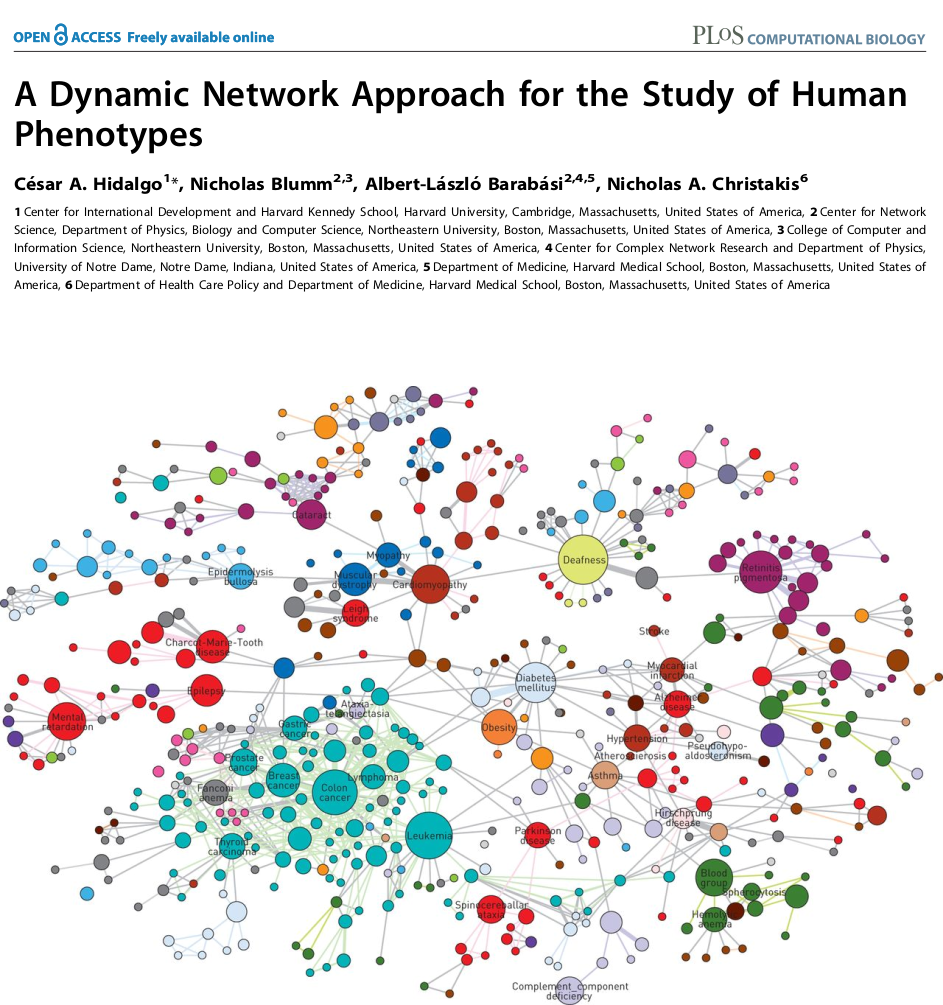
\includegraphics[keepaspectratio,width=0.5\textwidth]{images/HDN.png}

\end{frame}

\begin{frame}{Association rule mining}

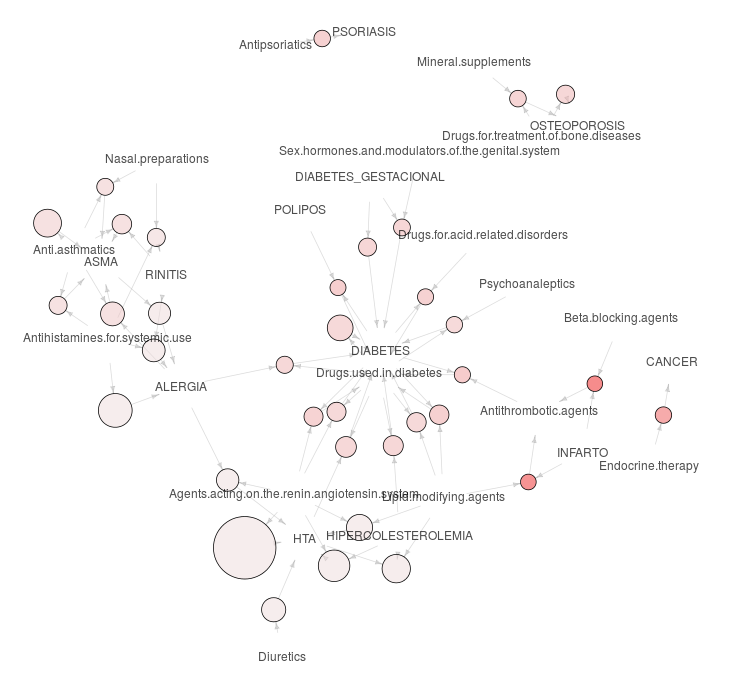
\includegraphics[keepaspectratio,width=0.5\textwidth]{images/rule_clusters.png}
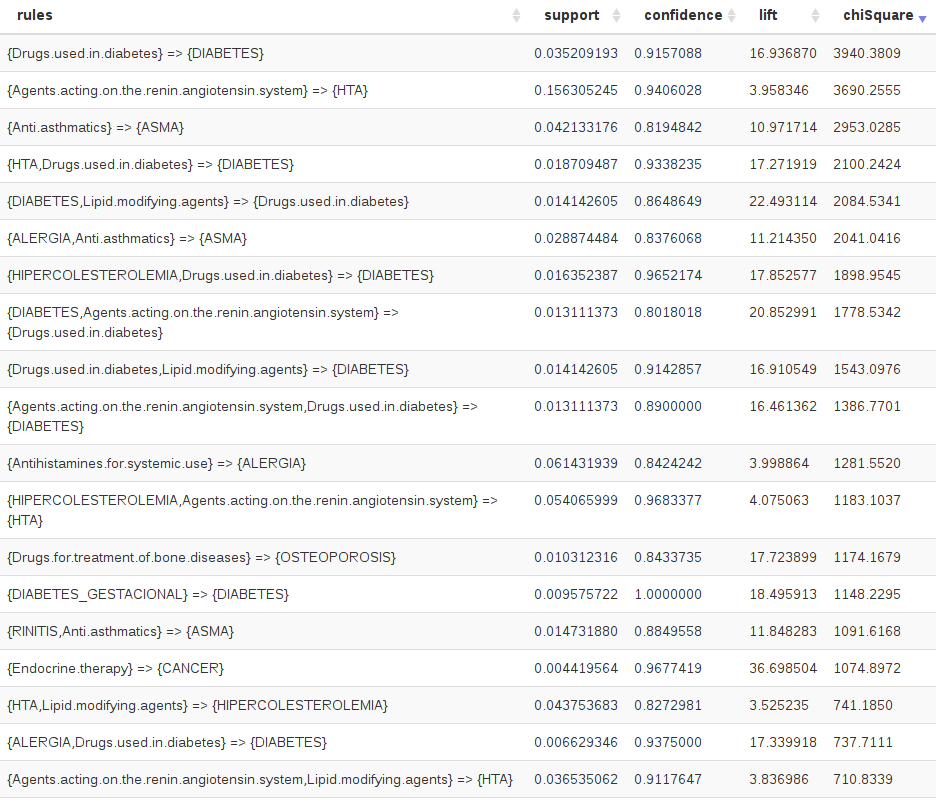
\includegraphics[keepaspectratio,width=0.5\textwidth]{images/rules.png}

Diseases and medications rule network from GCAT cohort

\end{frame}

\begin{frame}{Summary}

\begin{itemize}
\tightlist
\item
  Data-driven temporal analysis of the cohort
\item
  Identify subgroups of patients with distinct mechanisms of disease
\item
  Genome associations with disease subgroups
\item
  Risk models for common disorders
\item
  Stratified medicine
\end{itemize}

\end{frame}

\begin{frame}{Acknowledgements}

\begin{center}

\includegraphics[keepaspectratio,width=0.2\textwidth]{images/logo-GCAT.png}

Rafael de Cid, PhD


\includegraphics[keepaspectratio,width=0.8\textwidth]{images/larca.png}

Ricard Gavaldà, PhD

\end{center}

\end{frame}

\end{document}
